\documentclass{beamer}
\usepackage{amsmath}
\usetheme{Warsaw}
\definecolor{mygreen}{rgb}{.125,.5,.25}
\usecolortheme[named = mygreen]{structure}
\usepackage{graphicx}
\title{MATRIX PROJECT}
\subtitle{EE1390}
\author{Surya  Vijay}
\date{Feb-15-2019}

\begin{document}
\begin{frame}
\titlepage

\end{frame}

\begin{frame}[t]{PROBLEM }\vspace{10pt}
\begin{block}{Statement}
\ Let $p =   \begin{pmatrix}
    -1  ,& 0
              \end{pmatrix}
$
 $R=  \begin{pmatrix}
    3 ,& 3 \sqrt[]{3}
     \end{pmatrix}
     and \
   Q= \begin{pmatrix}
    0,&0
             
              \end{pmatrix} $
              be the points.the equation of the bisector of the angle PQR
\end{block}
\begin{figure}
   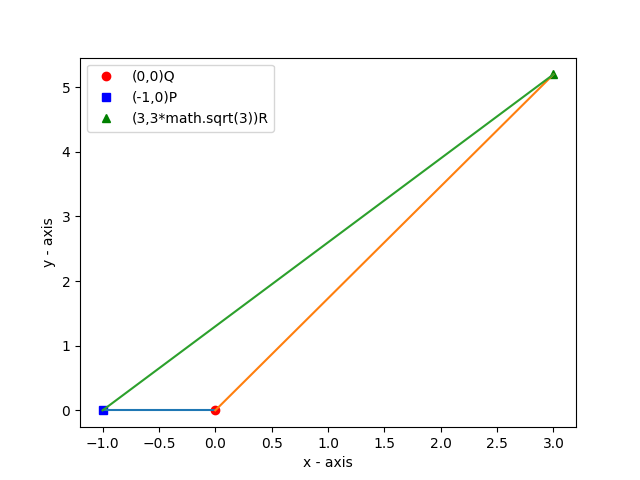
\includegraphics[scale=0.4]{Figure_1.png}
\end{figure}


\end{frame}



\begin{frame}[t]{Solution}

This method can be apllied for dividing the angle between two lines to n-times\\
\textbf{Steps:}\\[5.00mm] 
$ QP = \begin{pmatrix}
    -1  ,& 0
              \end{pmatrix} $ \\[5.00mm]  $
              QR = \begin{pmatrix}
    3 ,& 3 \sqrt[]{3}
     \end{pmatrix}
 $ \\[5.00mm] 
 $
  QR = \begin{pmatrix}
    1/2 ,&\sqrt[]{3} /2
     \end{pmatrix}
 $ -- Unit vector on the direction QR \\[5.00mm] 
 $ \begin{pmatrix}
      1/2 & \sqrt[]{3} /2
              \end{pmatrix} 
\begin{pmatrix}
     cos(x) & sin(x) \\-sin(x) & cos(x)
\end{pmatrix}  = \begin{pmatrix}
    -1,0
              \end{pmatrix} 
$
\\[5.00mm] 
Solving this we get $ x = 120^{o}$ 
\end{frame}
\begin{frame}{Solution}
angular bisector = 
$ \begin{pmatrix}
      1/2 & \sqrt[]{3} /2
              \end{pmatrix} 
\begin{pmatrix}
     cos(60^{o}) & sin(60^{o}) \\-sin(60^{o}) & cos(60^{o})
\end{pmatrix}  = \begin{pmatrix}
    -1/2 , \sqrt[]{3} /2
              \end{pmatrix} $
               \begin{figure}
   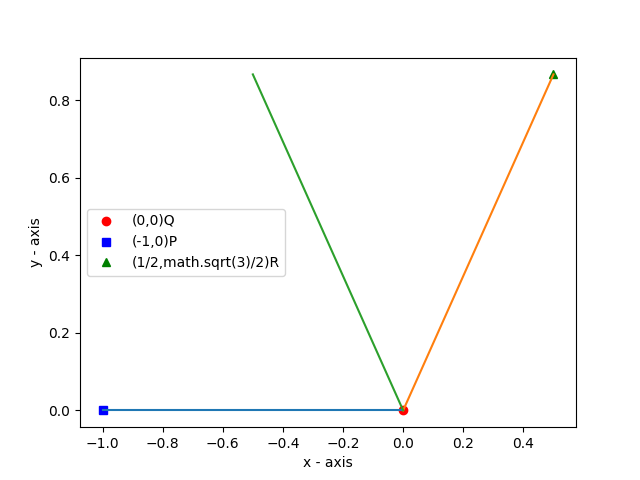
\includegraphics[scale=0.4]{Figure_2.png}
\end{figure}
\end{frame}
\begin{frame}{Solution2}
$ QP = \begin{pmatrix}
    -1  ,& 0
              \end{pmatrix} $ \\[5.00mm]  $
              QR = \begin{pmatrix}
    3 ,& 3 \sqrt[]{3}
     \end{pmatrix}
 $ \\[5.00mm] 
 $
  QR = \begin{pmatrix}
    1/2 ,&\sqrt[]{3} /2
     \end{pmatrix}
 $ -- Unit vector direction QR \\[3.00mm]
 Angular bisector angle is the made by unit vectors QP+QR
 \begin{figure}
   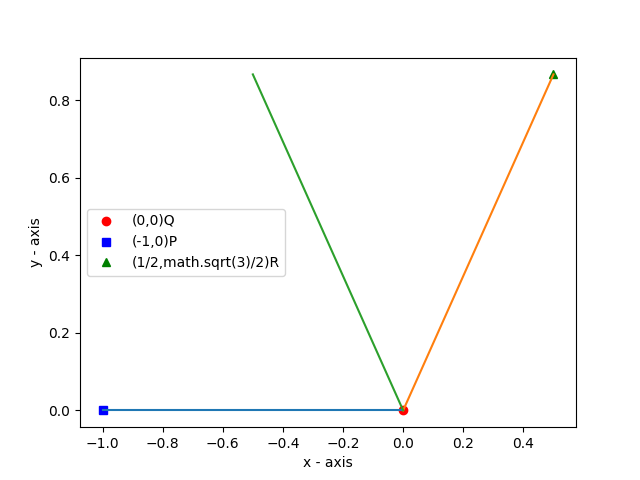
\includegraphics[scale=0.4]{Figure_2.png}
\end{figure}



\end{frame}
\end{document}

